
\documentclass[a4paper,fleqn,usenatbib,useAMS]{mnras}

\usepackage[utf8]{inputenc}

% Only include extra packages if you really need them. Common packages are:
\usepackage{graphicx}	% Including figure files
\usepackage{amsmath}	% Advanced maths commands
\usepackage{amssymb}	% Extra maths symbols
\usepackage{multicol}   % Multi-column entries in tables
\usepackage{bm}		    % Bold maths symbols, including upright Greek
%\usepackage{pdflscape}	% Landscape pages

\usepackage{newtxtext,newtxmath}
\usepackage[T1]{fontenc}
\usepackage{ae,aecompl}

\usepackage{subfig}
%%%%%%%%%%%%%%%%%%%%%%%%%%%%%%%%%%%%%%%
% \usepackage{xcolor}
% \definecolor{redak}{rgb}{0.9,0.15,0.05}
% \def \textred{\textcolor{redak}}
%%%%%%%%%%%%%%%%%%%%%%%%%%%%%%%%%%%%%%%
% \usepackage{epsfig}
% \usepackage{epstopdf}
% \usepackage{figsize}
% \usepackage{natbib}
%%%%%%%%%%%%%%%%%%%%%%%%%%%%%%%%%%%%%%%


\renewcommand{\vec}[1]{\mathbf{#1}}
\newcommand{\fracpartial}[2]{\frac{\partial #1}{\partial #2}}
\newcommand{\Lsun}{\mathrm{L_\odot}}
\newcommand{\ledd}{L_{\mathrm{Edd}}}
\newcommand{\Rsun}{\mathrm{R}_\odot}
\newcommand{\Msun}{\mathrm{M}_\odot}
% \newcommand{\lesim}{{<\atop{\sim}}}
\newcommand{\lesim}{\genfrac{}{}{0pt}{2}{<}{\sim}}
\newcommand{\tred}[1]{\textcolor{red}{#1}}
\newcommand{\tyellow}[1]{\colorbox{yellow}{#1}}
\newcommand{\ask}[1]{\textcolor{magenta}{#1}}
\newcommand{\emphbf}[1]{\textbf{\emph{#1}}}
% \newcommand{\myr}{\mathrm{M_\odot~yr^{-1}}}
\newcommand{\flash}[1]{\textsc{flash}#1}
\newcommand{\radmc}[1]{\textsc{radmc-3d}#1}
\newcommand{\yt}[1]{\texttt{yt}#1}
\newcommand{\visit}[1]{Visit#1}
\newcommand{\python}[1]{Python#1}

\def \kms{~\rm{km~s^{-1}}}
\def \kev{~\rm{keV}}
\def \eV{~\rm{eV}}
\def \cmcub{$\rm{cm}^{-3}$}
\def \msyr{~\rm{M_{\odot}}~\rm{yr^{-1}}}
\def \cm{~\rm{cm}}
\def \s{~\rm{s}}
\def \km{~\rm{km}}
\def \gm{\rm{gm}}
\def \K{~\rm{K}}
\def \g{~\rm{g}}
\def \G{~\rm{G}}
\def \AU{~\rm{AU}}
\def \erg{~\rm{erg}}
\def \yrs{~\rm{yrs}}
\def \yr{~\rm{yr}}
\def \pc{~\rm{pc}}
\def \kpc{~\rm{kpc}}
\def \etc{$\eta$~Car}
\def \days{~\rm{days}}
\def \Jy{~\rm{Jy}}
\def \mum{~\rm{\mu m}}
\def \keV{~\rm{keV}}
\def \astrobj#1{#1}
\def \rmModot{~\rm{M_{\sun}}}
\def \rmRodot{~\rm{R_{\sun}}}
\def \rmLodot{~\rm{L_{\sun}}}
% \def \rmMJ{~\rm{M_J}}
% \def \rmRJ{~\rm{R_J}}


\newcommand{\orcidAmit}{0000-0002-7840-0181}
\newcommand{\orcidAmir}{0000-0002-1361-9115}

% ==========================================================

\title[V838Mon 2002 eruption as an ILOT]{Radiation hydrodynamical simulations of the later phase of a merger-burst ILOT}
\author[A. Michaelis et al.]{
Amir Michaelis$^{1}$\thanks{E-mail: \href{mailto:amirmi@ariel.ac.il}{amirmi@ariel.ac.il}},
Amit Kashi$^{1}$\thanks{E-mail: \href{mailto:kashi@ariel.ac.il}{kashi@ariel.ac.il}}
\\
$^{1}$Department of Physics, Ariel University, Ariel, POB 3, 4070000, Israel \\
\\
}
\date{Accepted XXX. Received YYY; in original form ZZZ}
\pubyear{2020}

% ==========================================================
\begin{document}
\label{firstpage}
\pagerange{\pageref{firstpage}--\pageref{lastpage}}
\maketitle
\begin{abstract}
We simulate the later evolution of a merger-burst transient, consists of a massive thick accretion disc around a main sequence star.
The accretion disc is the result of probably a $1\Msun$ object on the verge of the main sequence distraction onto a $8\Msun$ star.
This setup emulate the properties of the prototype Luminous Red Nova, V838~Mon.
We find that XXXXMsun is accreted onto the star, and calculate the expected lightcurve.
We find XXXXXXXXX
\end{abstract}

\begin{keywords}
accretion, accretion discs --- (stars:) binaries: general
\end{keywords}

% ==========================================================
\section{Introduction}
\label{sec:intro}
V838~Mon is a well observed outburst first discovered January 2002 \citep{2002IAUC.7785....1B} to April 2002 \citep{2005A&A...436.1009T}.
It also include earlier time pregenerator \citep{2005A&A...441.1099T} and later time light echo observations \citep[for example][]{2018A&A...617A.129K}.
V838~Mon object is classified as luminous red nova and the leading model is of stellar merger \citep{2006A&A...451..223T,2014MNRAS.443.1319K,2015A&A...580A..34K,2016MNRAS.458..950S,2018A&A...617A.129K}.
Luminous Red Nova (LRN) or more accurate intermediate luminous red transient is a class of Intermediate Luminous Optical Transients \citep[ILOTs; recently also refereed to as ``Sokers'',][]{2016RAA....16...99K}.

LRN or Merger Bursts refer to quite diverse group of objects describing transients powered by a complete merger of two stars. 
The denser star is tidally destroys the less dense star and accretes most of its mass. This releases gravitational energy that powers the event. Some mass from the destroyed star escapes the system.
This presents a characteristic merger light curve. More object in this class are V1309~Sco \citep{2011A&A...528A.114T}, and possibly eruptions of somewhat more massive progenitors, NGC~4490-OT \citep{2016MNRAS.458..950S} and M101~OT2015-1 \citep{2017ApJ...834..107B} as well as the small young stellar object ASASSN-13db \citep{2019arXiv191207305K}.

The light curve declines by XXXX mag in XXXX days in the V-band.
SOKERYTLENDA calculated the bolometric light curve using a model XXXXXXTELL ABOUT IT.
They found that the peak luminosity is XXXX, and the total energy in the eruption is XXXXX.
XXXXX BOND? observed typical line velocities of XXXXkm/s.
More obs.XXXX


If we use V838~Mon as the prototype of its class od light curves, we see that the rise time scale is in the order of days and can have more then one stage. We expect to have more than one peak. The decline stage is very steep, occasionally with local peaks along the decline \citep{2003MNRAS.341..785C,2005MNRAS.358.1352C}.
\cite{2006A&A...451..223T} argued that this behaviour best fits by gravitational dominated process.
\cite{2010ApJ...709L..11K} showed that V838~Mon and many other transients have similar shapes of their light curves when scaling the time axis.
Moreover, these authors suggested to classify transients by estimating the total energy of each event (radiation $+$ kinetic energy) rather than by the peak of its light curve.
%(the practice that was commonly used before than e.g. \citealt{2007Natur.447..458K}).
The Energy-Time Diagram (ETD) is used for that purpose \citep{2016RAA....16...99K,2017MNRAS.468.4938K} \footnote{For an up-to-date ETD figure see \url{phsites.technion.ac.il/soker/ilot-club/} }.
In the EDT many of the transients form a slated stripe more energetic than novae yet less energetic than SNe, referred to as the Optical Transient Stripe (OTS).


CITE XXXX SOKER TYLENDA suggested a model a model for the observation of LRNe is stellar merger see ....
The merger in this system a massive star with a regular star where the accreted star is less dens probably a YSO with thick accretion disk.
The probably result in massive star with thick disk see...




describe creation of thick disk (cooling time and viscosity longer the Keplerian and dynamic time) from frank power accretion (FKR)
Tidal disruption radius and time \citep{1988Natur.333..523R}.

In this paper we model the system as merger resulting thick accretion disk around massive star.
We focus on the accretion process and resulting observational signature expected (light curve) from such system.
and discuss V838~Mon observation in light of this analysis.


XXXX velocity of matter eject ot of the photosphere of the disk relative to observations (and spectrums).
XXXX more quotes and description specific to V838~Mon


% ==========================================================
\section{Model}
\label{sec:model}

using flash.
setup physical details (disk mass radios and ext...)
initial density (disk alpha angle),temperature,energy profile
the simple analytical model from FKR \cite{2002apa..book.....F} and Abramowicz(1990?) \cite{1988MNRAS.232....1F,1991ApJ...370L..35A}  ....
initial condition and boundary condition (adjust simulation)
how to simulate the accreted matter.
RadMC-3D to create spectrum (SED) and light curve
RadMC-3D model chosen
describe the process of creating light curve from spectrum
XXX Mention the start in the center is not part of the simulation.
%%%%%%%%
\begin{figure}
    \begin{center}
    \subfloat[Slice view \label{subfig:slice}]{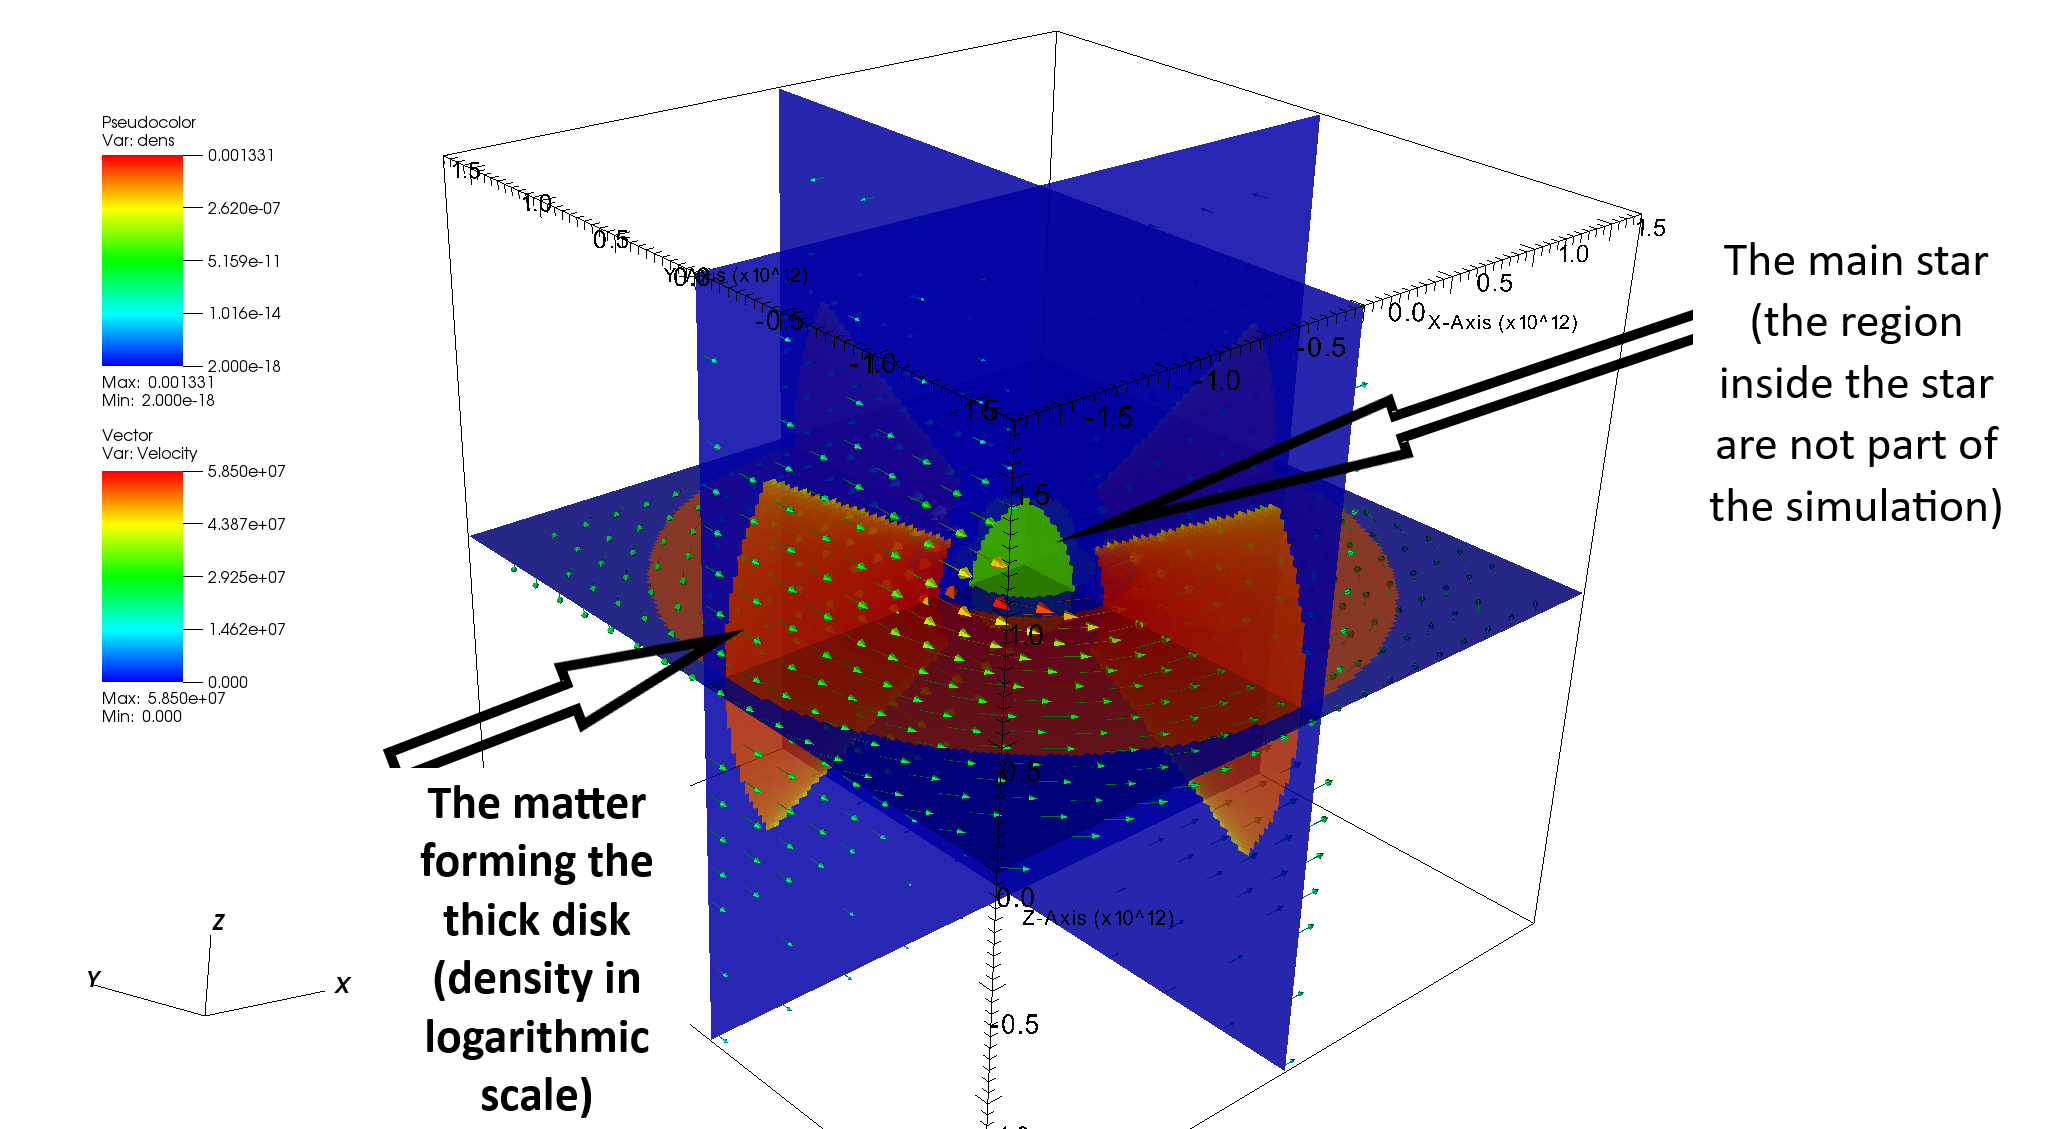
\includegraphics[width=0.5\textwidth]{initial_condition_slice3_annotation.png}} \\
    \subfloat[Volume view \label{subfig:3d}]{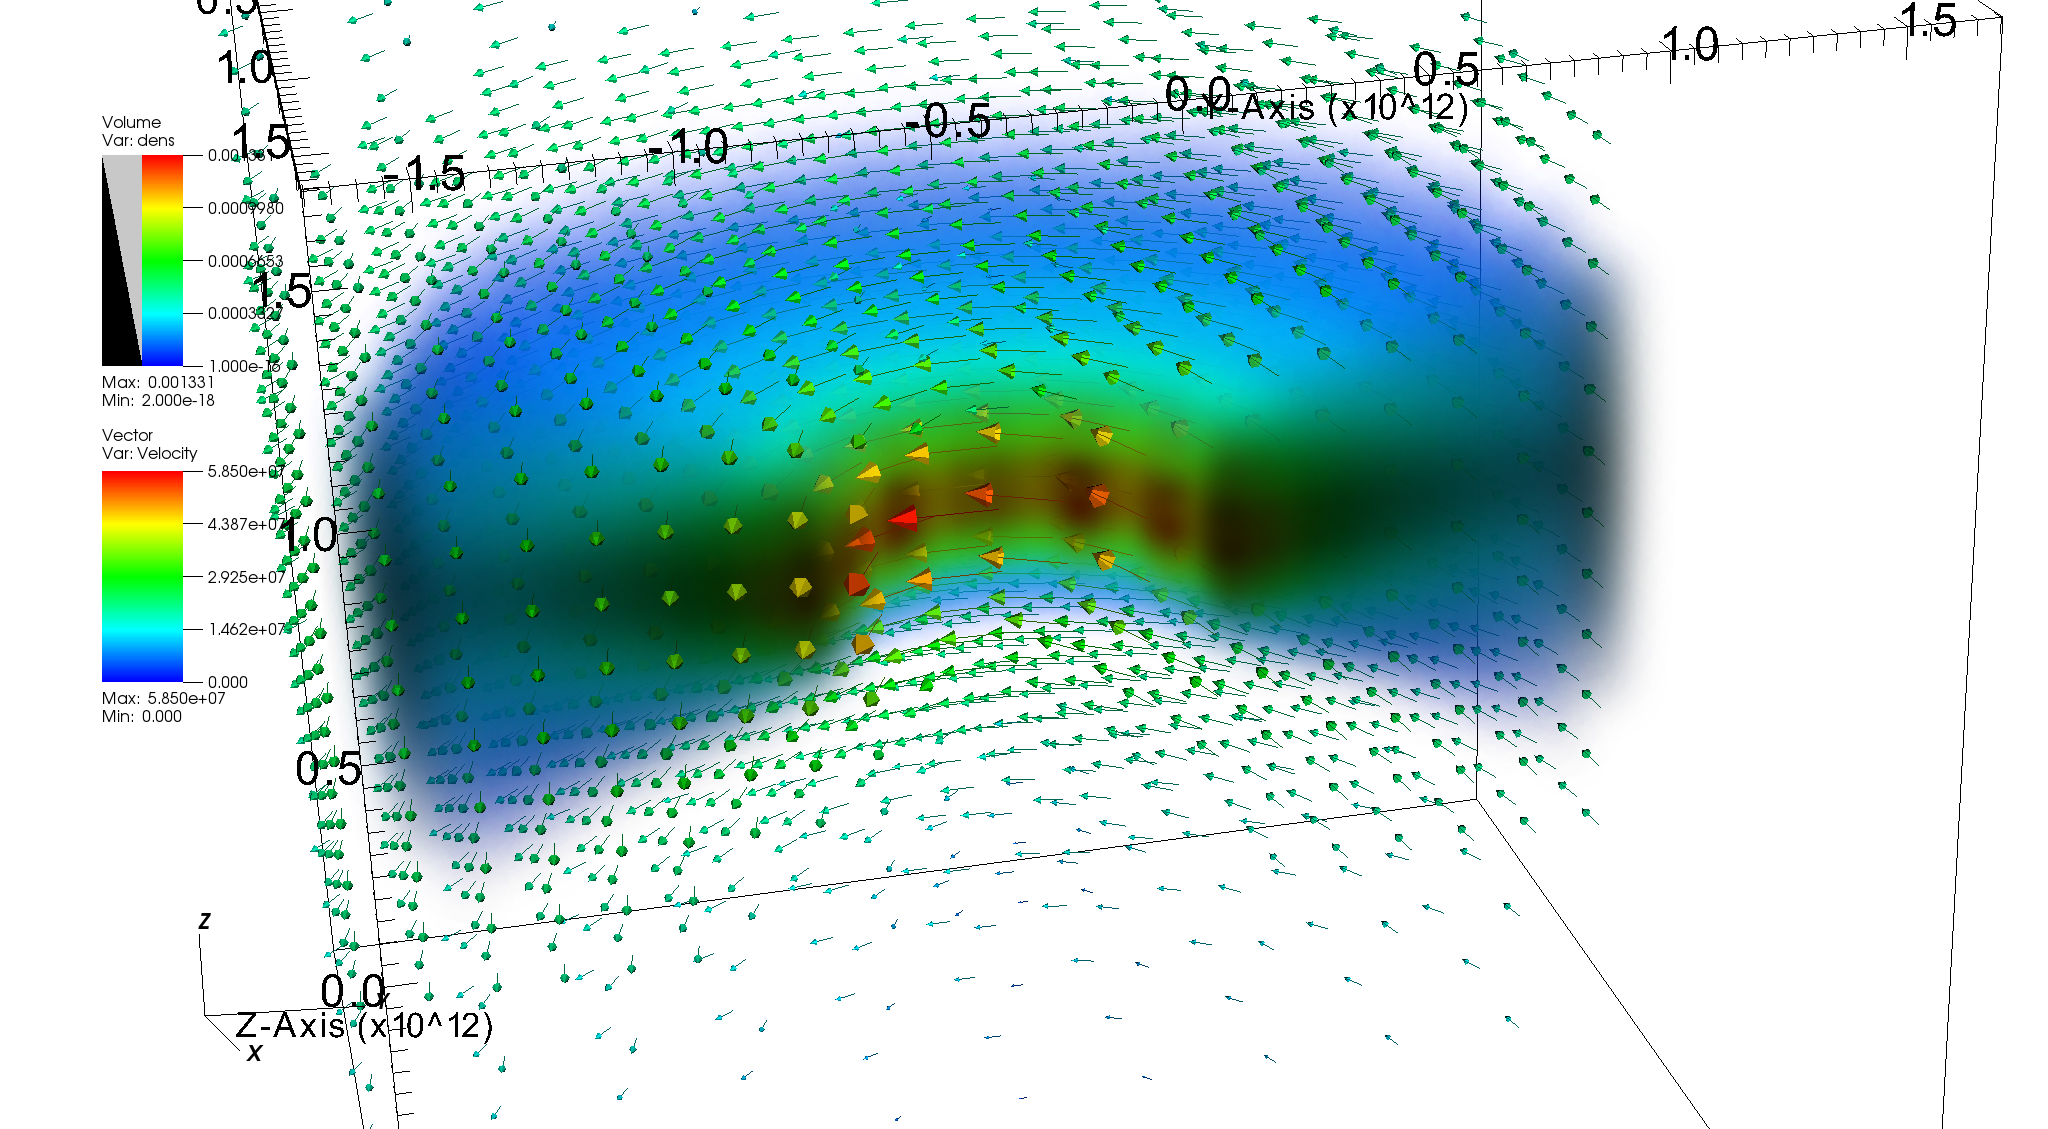
\includegraphics[width=0.5\textwidth]{initial_condition_3d.png}}
    \end{center}
    \caption{
        The initial density and velocity. 
        In \ref{subfig:slice} we see the density along the x-y, x-z and y-z plane in logarithmic scale and the velocity. 
        The angle of the thick disk $\alpha=30^\circ$. 
        We use the star in the center as a boundary condition.
        In \ref{subfig:3d} we see the initial density voxel in linear scale and the velocity. 
        }
    \label{fig:initial_condition}
\end{figure}
%%%%%%%%

XXXX Fig for initial setup.

% ==========================================================
\section{Results}
\label{sec:results}
We run the simulation with these parameters ... 
on a cluster  ...
show graphs on matter and accretion ....
accretion rate?
%%%%%%%%
\begin{figure}
    \begin{center}
        \subfloat[Accretion \label{subfig:slice}]{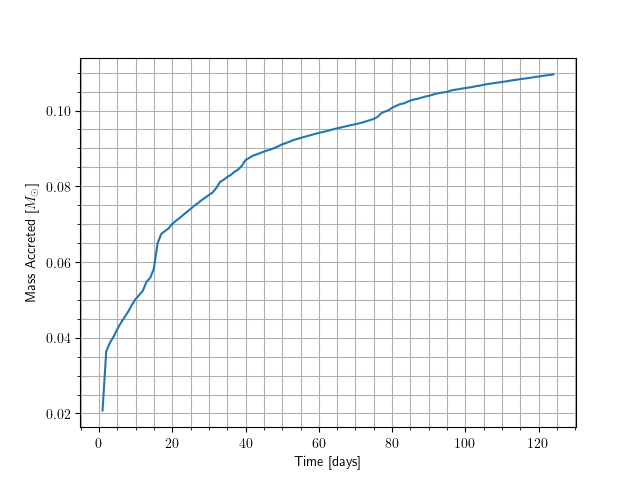
\includegraphics[width=0.5\textwidth]{accretion.png}} \\
        \subfloat[Accretion rate \label{subfig:3d}]{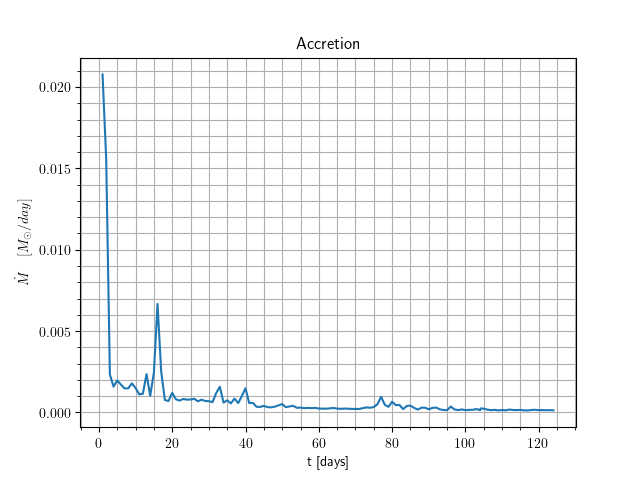
\includegraphics[width=0.5\textwidth]{acc_mdot.png}}
    \end{center}
    \caption{
        accretion rate
        }
    \label{fig:accretion_rate}
\end{figure}
%%%%%%%%

%%%%%%%%
\begin{figure}
    \begin{center}
        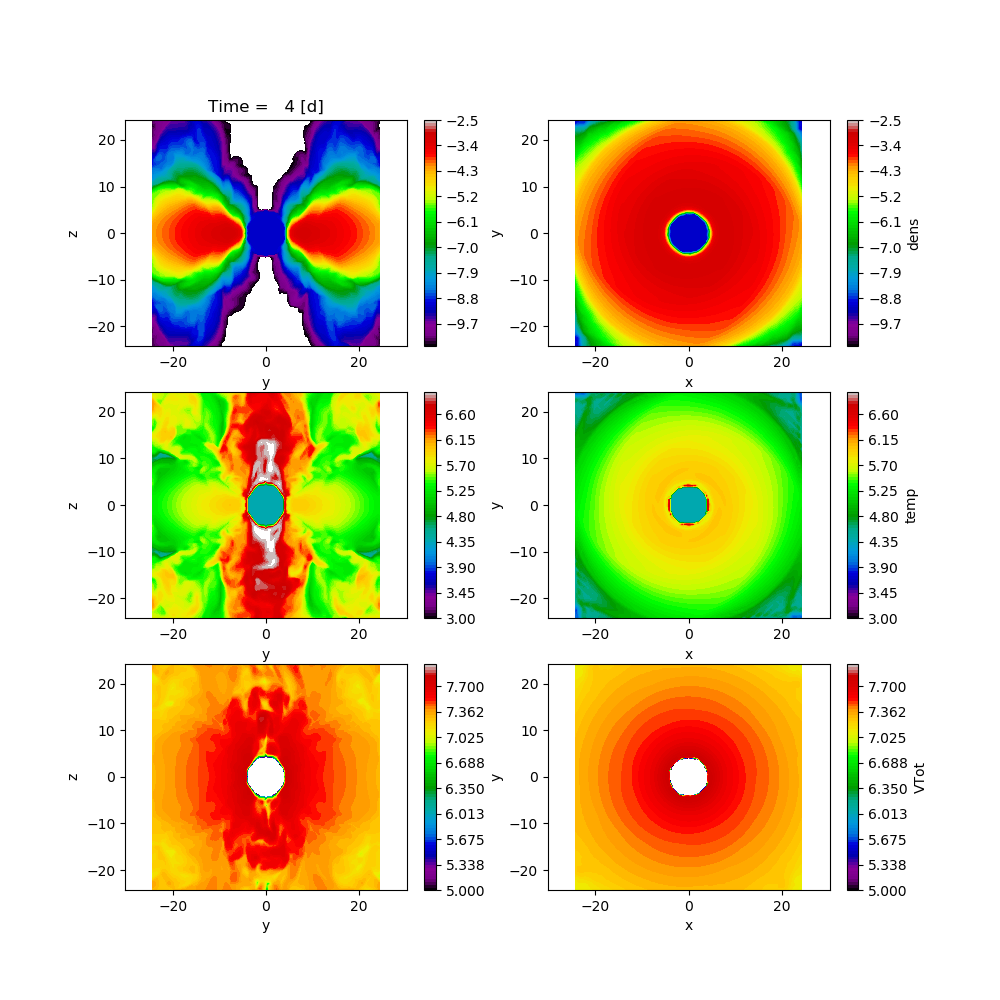
\includegraphics[width=0.5\textwidth]{disk_hdf5_chk_0005_slice.png}
    \end{center}
    \caption{
        Slice view of the disk in time t
        }
    \label{fig:disk_chk_slice}
\end{figure}
%%%%%%%%

%%%%%%%%
\begin{figure}
    \begin{center}
        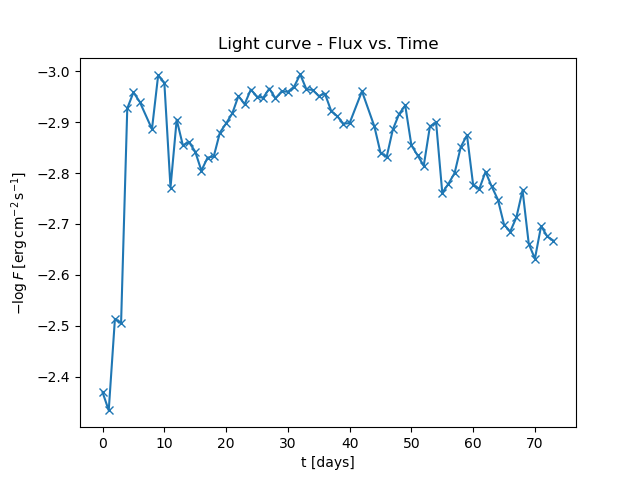
\includegraphics[width=0.5\textwidth]{light_curve.png}
    \end{center}
    \caption{
        Light curve
        }
    \label{fig:light-curve}
\end{figure}
%%%%%%%%

show graphs on spectrum and light curve (RadMC-3D results) with the following inc angle (0,30,60,90) + obs of bolometric light curve of V838~MON

discuss the first few days instability !

% ==========================================================
\section{Discussion}
\label{sec:discuss}
analysis of the relation of the result with the expected observation of V838 Mon
discus the influence of the different parameter to the model
what we expect and what we received

XXXXX compare velocities of lines from obs to velocities in the simulation. Figure
Discuss the first few days numeric Rayleigh-Taylor instability and shock waves
% ==========================================================
\section{Conclusions}
\label{sec:concl}
what dose it say using this model in for such observation (thick disk model of accretion for red nova)


% ==========================================================
\section{Acknowledgements}
\label{sec:acknow}
compute canada
ariel university (scholar ship and ext...)
Noam???

% ==========================================================
\bibliographystyle{mnras}
\bibliography{bibdb}
% ==========================================================
\label{lastpage}
\end{document}
